\subsection{High-dimensional datasets and small \texorpdfstring{$k$}{k}}
\label{sec:boundary}

On real data CIF ranks lowest at small $k$ and on wide datasets. At small $k$
it ranks 7th or 8th of 17 in classification on the complete-case panel
(\cref{fig:k-trajectory}). On wide datasets its scores peak before the full
feature set. Across the 15 classification datasets with more than 100
features, CIF first reaches its best score at an intermediate value of $k$
($100 < k < p$) in 29 of 45 dataset-learner combinations, and at the full
feature set ($k=p$) in 7 of 45.

\Cref{fig:high-p-boundary} shows this pattern by downstream learner. Scores
peak at intermediate $k$ on 8 of 15 LR datasets, 12 of 15 SVM datasets, and 9
of 15 KNN datasets. The full feature set helps mainly LR. Moving
from $k=100$ to $k=p$ changes the LR score by $+0.026$ on average, and LR first
reaches its best score at $k=p$ on 5 of 15 datasets. For SVM and KNN the mean
changes are $-0.053$ and $-0.071$.

In the 6 high-dimensional regression datasets, full-feature evaluation is
rarely best. Of the 18 dataset-learner combinations, 12 peak at or below
$k=100$ and 2 at $k=p$. The change from $k=100$ to $k=p$ has a mean of
$-0.270$ and a median of $-0.076$.

\begin{figure}[!htbp]
  \centering
  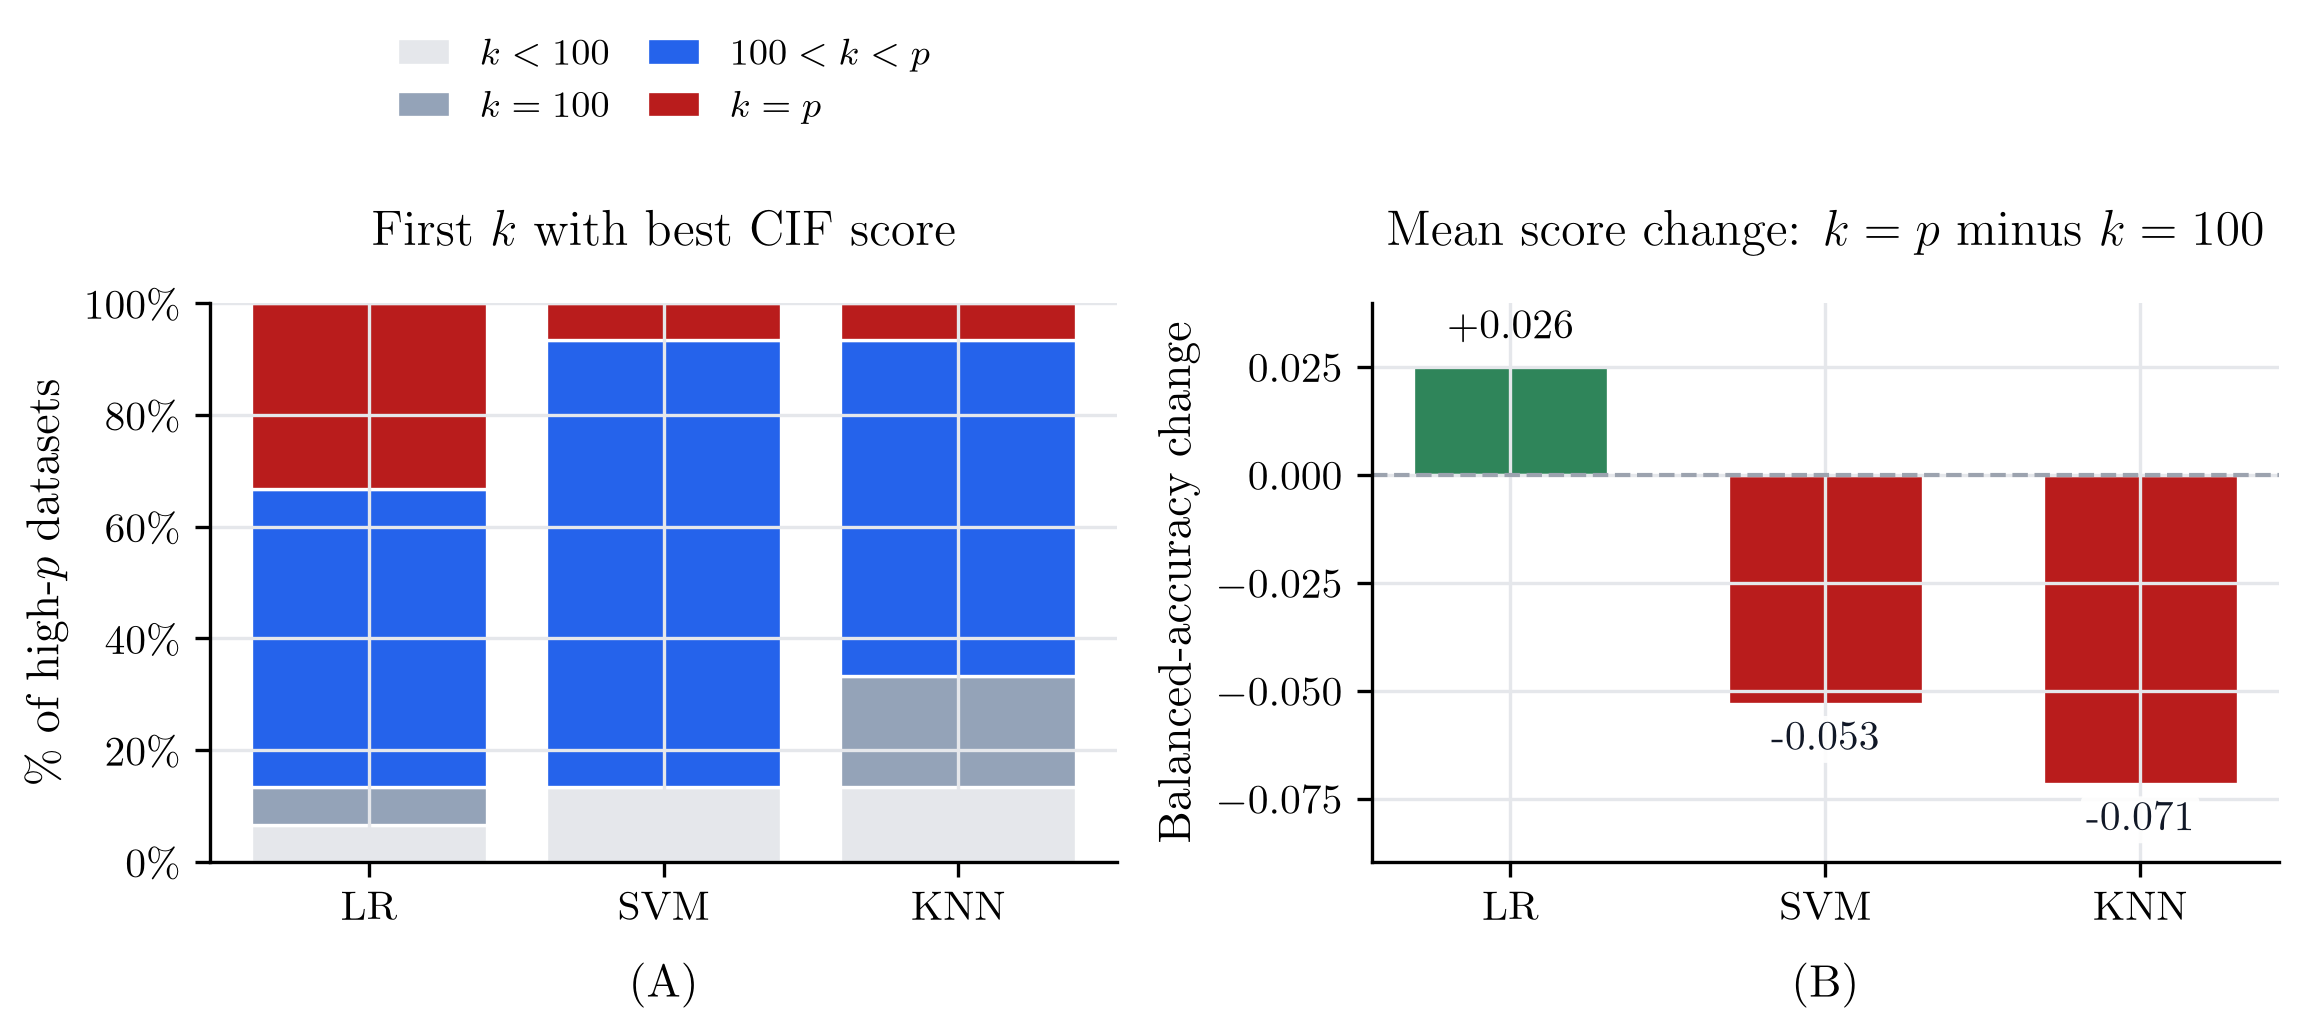
\includegraphics[width=0.84\linewidth]{figures/high_p_boundary_summary.png}
  \caption{Where CIF's classification scores peak as $k$ increases, by
  downstream learner. (A) shows, for each learner, the percentage of 15
  datasets where the first evaluated $k$ attaining the best observed CIF score
  falls below 100, at 100, between 100 and $p$, or at $k=p$. (B) shows the mean
  balanced accuracy change from $k=100$ to $k=p$.}
  \label{fig:high-p-boundary}
\end{figure}

\subsection{Synthetic recovery}
\label{sec:synthetic-recovery}

On synthetic datasets with known informative features, CIF sits at or below
the median position of the methods run on each task
(\cref{tab:synthetic-head}). It recovers true features within the top-$k$ list
more reliably than it places one first. On the redundant-feature designs,
where correlated copies of informative features count as hits, CIF ranks 1st
of 16 in regression and tied 7th of 15 in classification.
\Cref{fig:synthetic-topk-curves} shows recovery as $k$ grows.

\begin{table}[!htbp]
  \centering
  \footnotesize
  \setlength{\tabcolsep}{6pt}
  \begin{tabular}{@{}lcccc@{}}
    \toprule
    & \multicolumn{2}{c}{Classification} & \multicolumn{2}{c}{Regression} \\
    \cmidrule(lr){2-3}\cmidrule(l){4-5}
    \tablehead{Metric} & {Value} & Rank & {Value} & Rank \\
    \midrule
    Selected features that are informative & 35.3\% & \countfrac{8}{15} & 39.1\% & \countfrac{11}{16} \\
    Top-1 hit rate & 65.5\% & \countfrac{10}{15} & 84.5\% & \countfrac{10}{16} \\
    True or redundant (redundant design only) & 82.4\% & \countfrac{7.5}{15} & 83.8\% & \countfrac{1}{16} \\
    \bottomrule
  \end{tabular}
  \caption{Synthetic feature recovery for CIF. The first row averages, over
  $k = 5, 10, 25, 50$, and $100$, the percentage of selected features that are
  truly informative. The top-1 hit rate is computed at $k=1$. The final row is
  computed and ranked only on the redundant-feature design for each task and
  counts true informative plus redundant features. Ranks are among the 15
  classification and 16 regression methods with synthetic runs; fractional
  ranks indicate averaged ties.}
  \label{tab:synthetic-head}
\end{table}

\begin{figure}[!htbp]
  \centering
  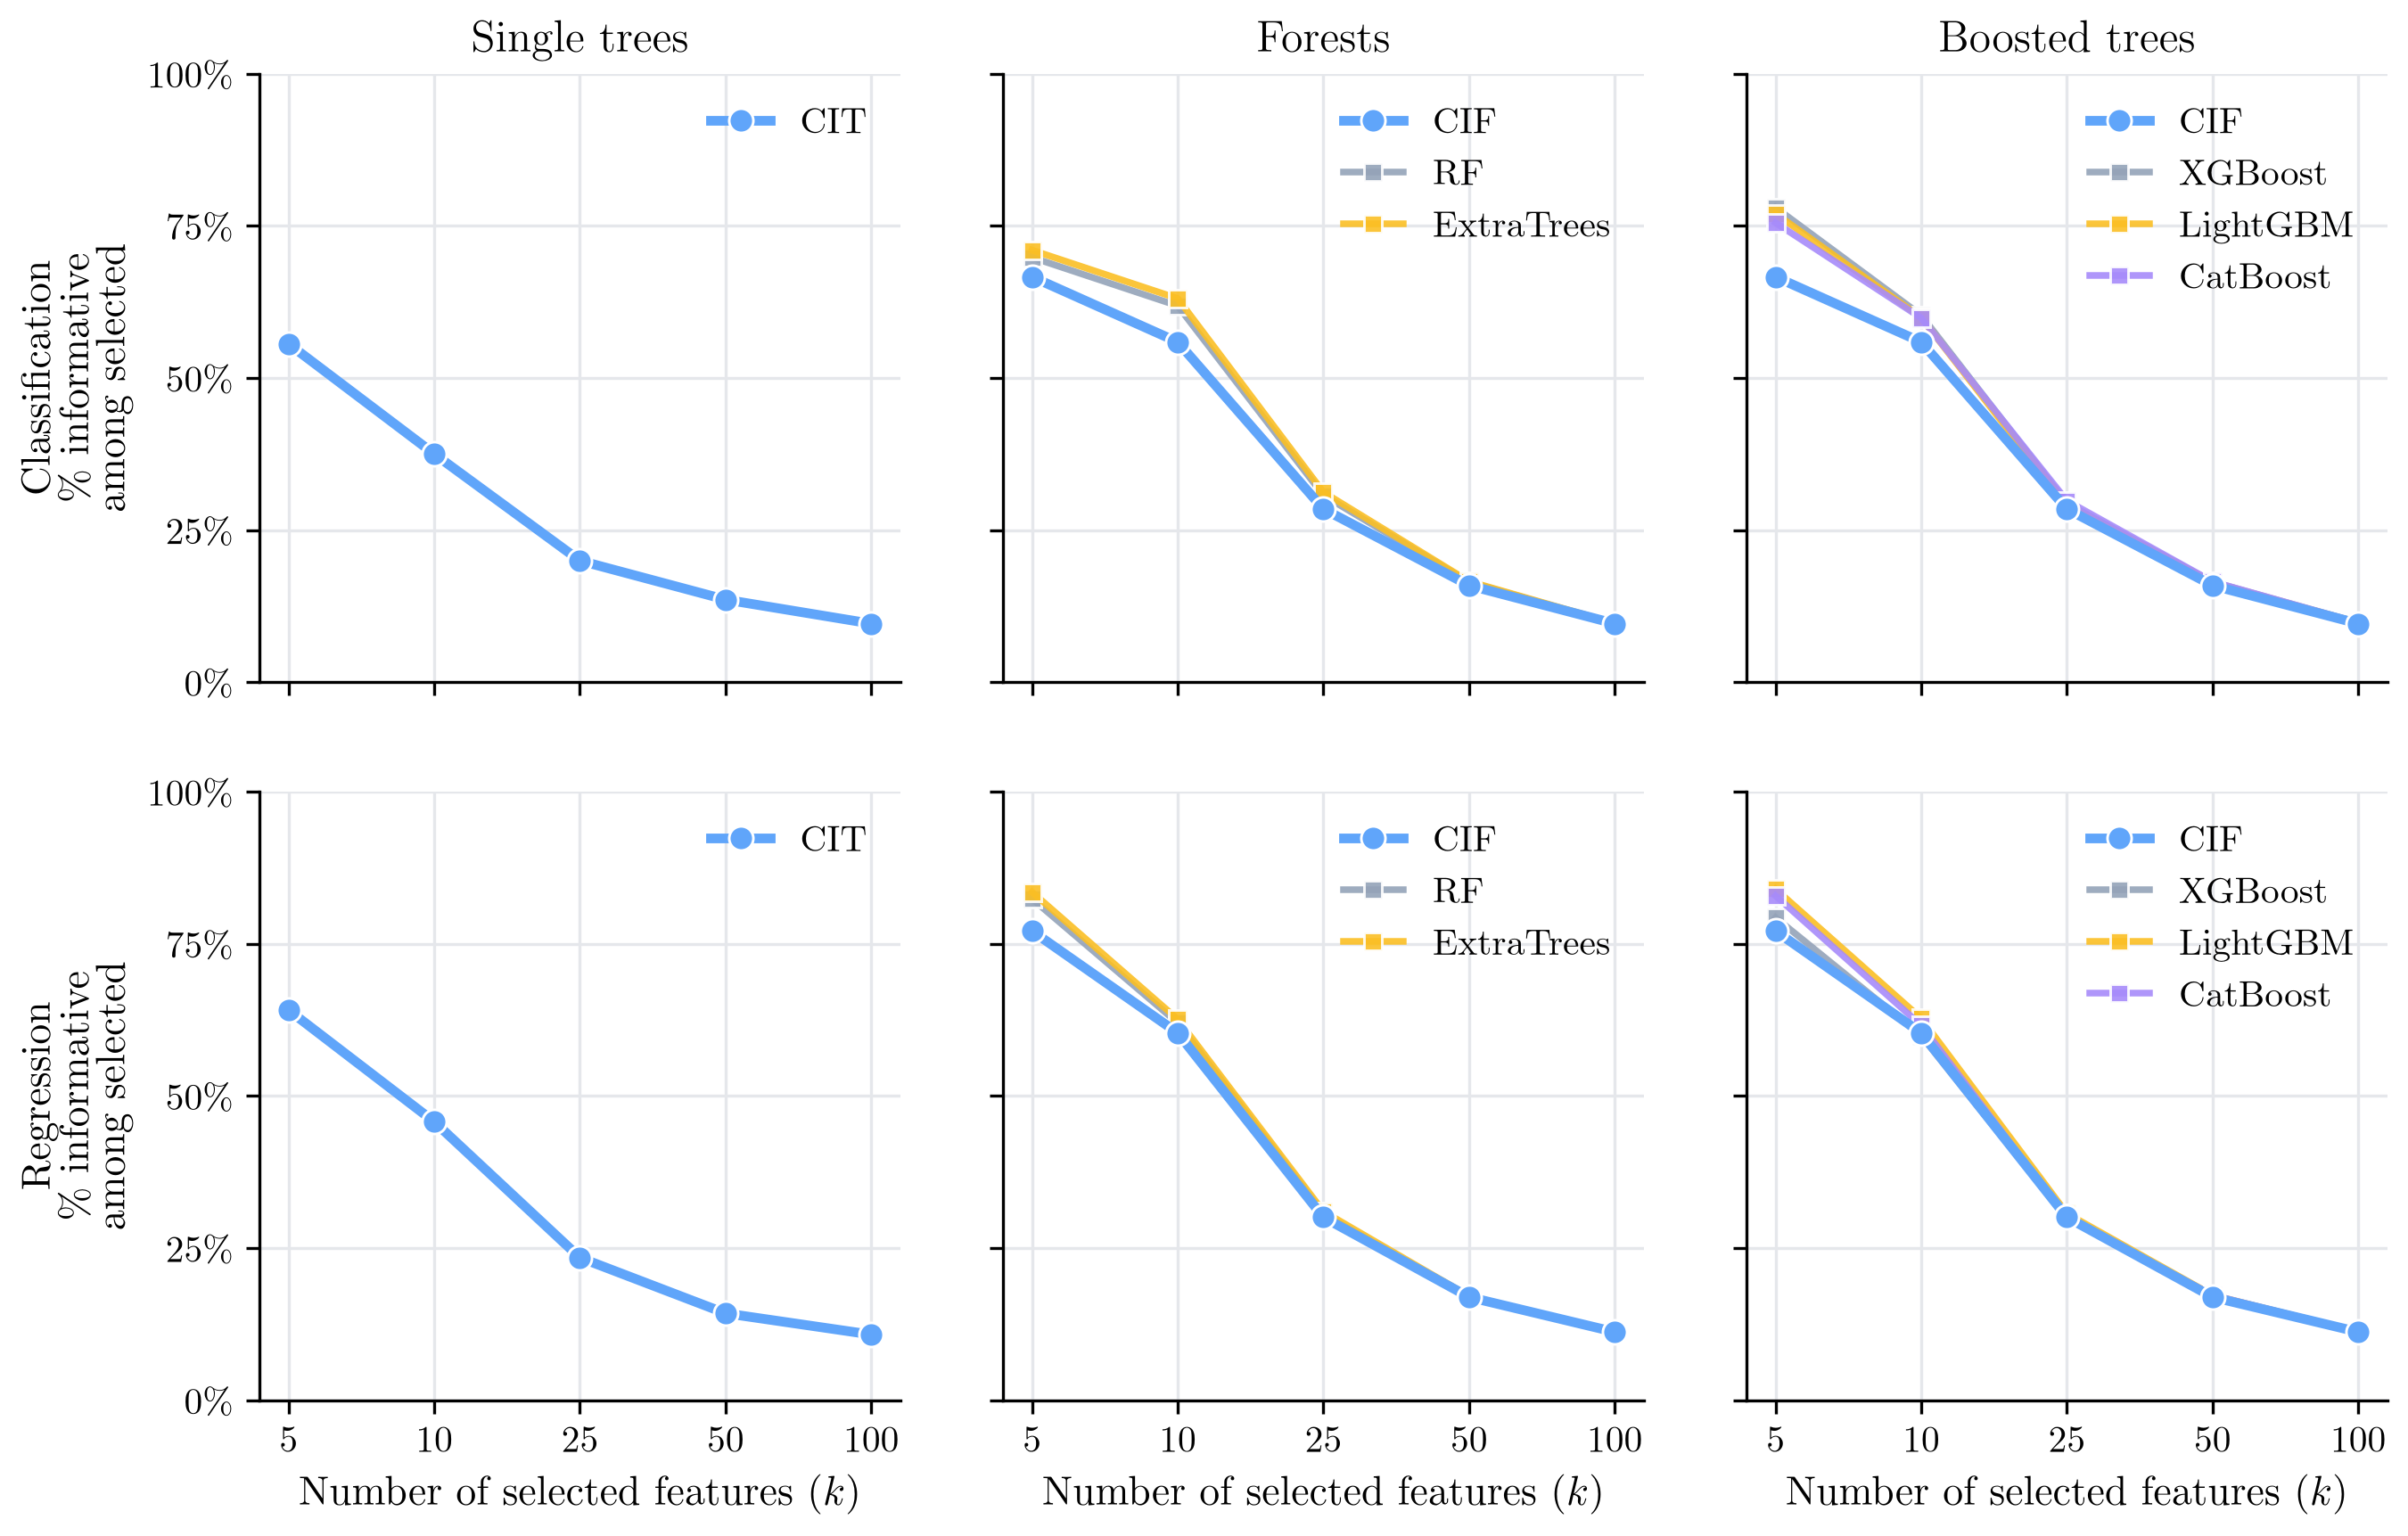
\includegraphics[width=0.84\linewidth]{figures/synthetic_topk_focus_curves.png}
  \caption{Synthetic top-$k$ recovery curves. Columns compare single trees,
  forests, and boosted trees; rows show classification and regression. Each
  value is the percentage of selected features that are truly informative.}
  \label{fig:synthetic-topk-curves}
\end{figure}

\subsection{Mechanism: cardinality and feature use}
\label{sec:mechanism}

Three measurements examine how the split rule shapes a ranking. They cover the
preference for high-cardinality features, the size of each ranker's support,
and the limit that feature sampling places on which features a forest can
split on.

\paragraph{Cardinality in the ranking.}
The weak-signal designs place 10 informative Gaussian features among
500-level, binary, and Gaussian noise columns
(\cref{tab:weak-signal-cardinality}). A ranker indifferent to cardinality would
give each of the 500-level and binary noise types 25/60 of the top-ten places
not taken by informative features. The designs can reveal two biases, and both
appear. The first is the preference of impurity importance for features with
many possible thresholds; the second is the reverse cardinality bias of the
per-threshold rule (\cref{sec:rank-construction}). At the weakest signal, random forest impurity importance fills
0.38 of its top ten with 500-level noise in both tasks, against a reference of
0.24, and none with binary noise. Per-threshold CIF is close to the reference
in classification (0.31 binary and 0.26 500-level against 0.29) and leans
toward binary noise in regression (0.40 binary and 0.24 500-level against
0.31). The max-type rule brings the binary share to 0.26 in classification and
0.30 in regression, against references of 0.28 and 0.27.

A ranking with less cardinality preference does not recover more informative
features in these designs. Random forest impurity
importance places the most informative features in its top ten at every signal
strength, and the downstream scores of all rankers are within 0.02 of each
other at every signal. The same forest ranked by out-of-bag permutation
importance keeps the preference, with a 500-level share above that of
impurity importance at the two weaker signals in both tasks. The benefit of a
ranking closer to cardinality-neutral appears on predictors whose cardinality
carries no signal, as in the clinical application of
\citet{MilletichDownesHirst2026citrees}, rather than in recovery of weak
marginal effects.

\begin{table}[!htbp]
  \centering
  \footnotesize
  \setlength{\tabcolsep}{5pt}
  \begin{tabular}{@{}lrlrrrrr@{}}
    \toprule
     & & & \multicolumn{3}{c}{Share of the top ten} & & \\
    \tablehead{Task} & Signal & Ranking & Informative & 500-level noise & Binary noise & Support & Score \\
    \midrule

    Classification & 0.05 & CIF & 0.31 & 0.26 & 0.31 & 37 & 0.52 \\
     & & CIF, max-type & 0.34 & 0.28 & 0.26 & 46 & 0.51 \\
     & & RF impurity & 0.42 & 0.38 & 0.00 & 70 & 0.52 \\
     & & RF permutation & 0.30 & 0.47 & 0.06 & 34 & 0.51 \\
     & 0.10 & CIF & 0.64 & 0.16 & 0.13 & 45 & 0.56 \\
     & & CIF, max-type & 0.66 & 0.20 & 0.06 & 53 & 0.55 \\
     & & RF impurity & 0.72 & 0.19 & 0.00 & 70 & 0.56 \\
     & & RF permutation & 0.49 & 0.36 & 0.02 & 36 & 0.56 \\
     & 0.20 & CIF & 0.95 & 0.04 & 0.01 & 59 & 0.68 \\
     & & CIF, max-type & 0.96 & 0.04 & 0.00 & 65 & 0.69 \\
     & & RF impurity & 0.99 & 0.01 & 0.00 & 70 & 0.69 \\
     & & RF permutation & 0.87 & 0.09 & 0.00 & 39 & 0.67 \\
    Regression & 0.05 & CIF & 0.26 & 0.24 & 0.40 & 17 & $-$0.11 \\
     & & CIF, max-type & 0.34 & 0.22 & 0.30 & 21 & $-$0.11 \\
     & & RF impurity & 0.43 & 0.38 & 0.00 & 70 & $-$0.11 \\
     & & RF permutation & 0.37 & 0.43 & 0.05 & 34 & $-$0.10 \\
     & 0.10 & CIF & 0.64 & 0.11 & 0.20 & 24 & $-$0.05 \\
     & & CIF, max-type & 0.65 & 0.13 & 0.15 & 28 & $-$0.04 \\
     & & RF impurity & 0.73 & 0.17 & 0.00 & 70 & $-$0.04 \\
     & & RF permutation & 0.57 & 0.27 & 0.01 & 37 & $-$0.06 \\
     & 0.20 & CIF & 0.95 & 0.03 & 0.02 & 36 & 0.28 \\
     & & CIF, max-type & 0.95 & 0.02 & 0.02 & 44 & 0.28 \\
     & & RF impurity & 0.99 & 0.01 & 0.00 & 70 & 0.29 \\
     & & RF permutation & 0.95 & 0.03 & 0.00 & 39 & 0.28 \\
        \bottomrule
  \end{tabular}
  \caption{Weak-signal designs with mixed-cardinality noise, $n = 1{,}000$.
  Ten informative standard normal features have marginal correlation with the
  response given by the Signal column; the noise is 25 columns of integer codes
  on 500 levels, 25 binary columns, and 10 Gaussian columns. Shares are the mean
  composition of each ranking's top ten over 25 fits (5 seeds by 5 folds;
  standard errors 0.01 to 0.03); the remainder is Gaussian noise. Support is
  the mean number of features with nonzero importance; Score is the held-out
  balanced accuracy or $R^2$ of the downstream learners on the top ten. CIF is
  the selected configuration with the MC selector in classification and the PC
  selector in regression; CIF, max-type adds the max-type Stage~B rule; RF
  permutation is the same random forest ranked by out-of-bag permutation
  importance.}
  \label{tab:weak-signal-cardinality}
\end{table}

\paragraph{Support.}
The support of a ranker is the set of features that win at least one split.
On the synthetic datasets, random forests give every feature nonzero
importance on 15 of the 16 designs, and 800 of 1,000 on the 1,000-feature
classification design. On 13 of the 16 designs, CIF's support keeps 90 to
100\% of the planted features, so the support serves as a shortlist. Beyond it, a
ranking orders the zero-importance features by the tie rule of
\cref{sec:rank-construction}. For a single tree these filler features are most
of any top-$k$ list. They make up 52, 81, and 90\% of the CIT top 10, 25, and
50 features, against 0, 3, and 14\% for CIF and none for random forests. This is
consistent with single trees ranking near the bottom of the benchmark.

\paragraph{Feature use in sampled forests.}
A sparse simulation measures how often forest splits use informative features
(\cref{fig:candidate-forest-counts}; \cref{app:candidate-availability}). CIT
uses informative features in 100.0\% of classification splits and 93.5\% of
regression splits. Over the 12 classification forest designs, CIF uses
informative features in 33.2\% of splits, against 91.7\% for CIF-all, 8.4\%
for RF, and 6.5\% for ExtraTrees. RF and ExtraTrees grow to purity, so most of
their splits are deep splits on noise, while CIF stops at the permutation
test. The gap to CIF-all reflects feature sampling. With 32 of 1,000 features
sampled at a node and two informative, an informative feature is a candidate
at 6.3\% of nodes. In that design CIF uses one in 9.0\% of splits, RF in 2.7\%,
ExtraTrees in 2.0\%, and CIF-all in 100.0\%. When the sampled subset holds no
informative feature, Stage~A selects from the noise it was given. The
downstream ranking of CIF-all was not scored, so its effect on ranking quality
remains open.

\begin{figure}[!htbp]
  \centering
  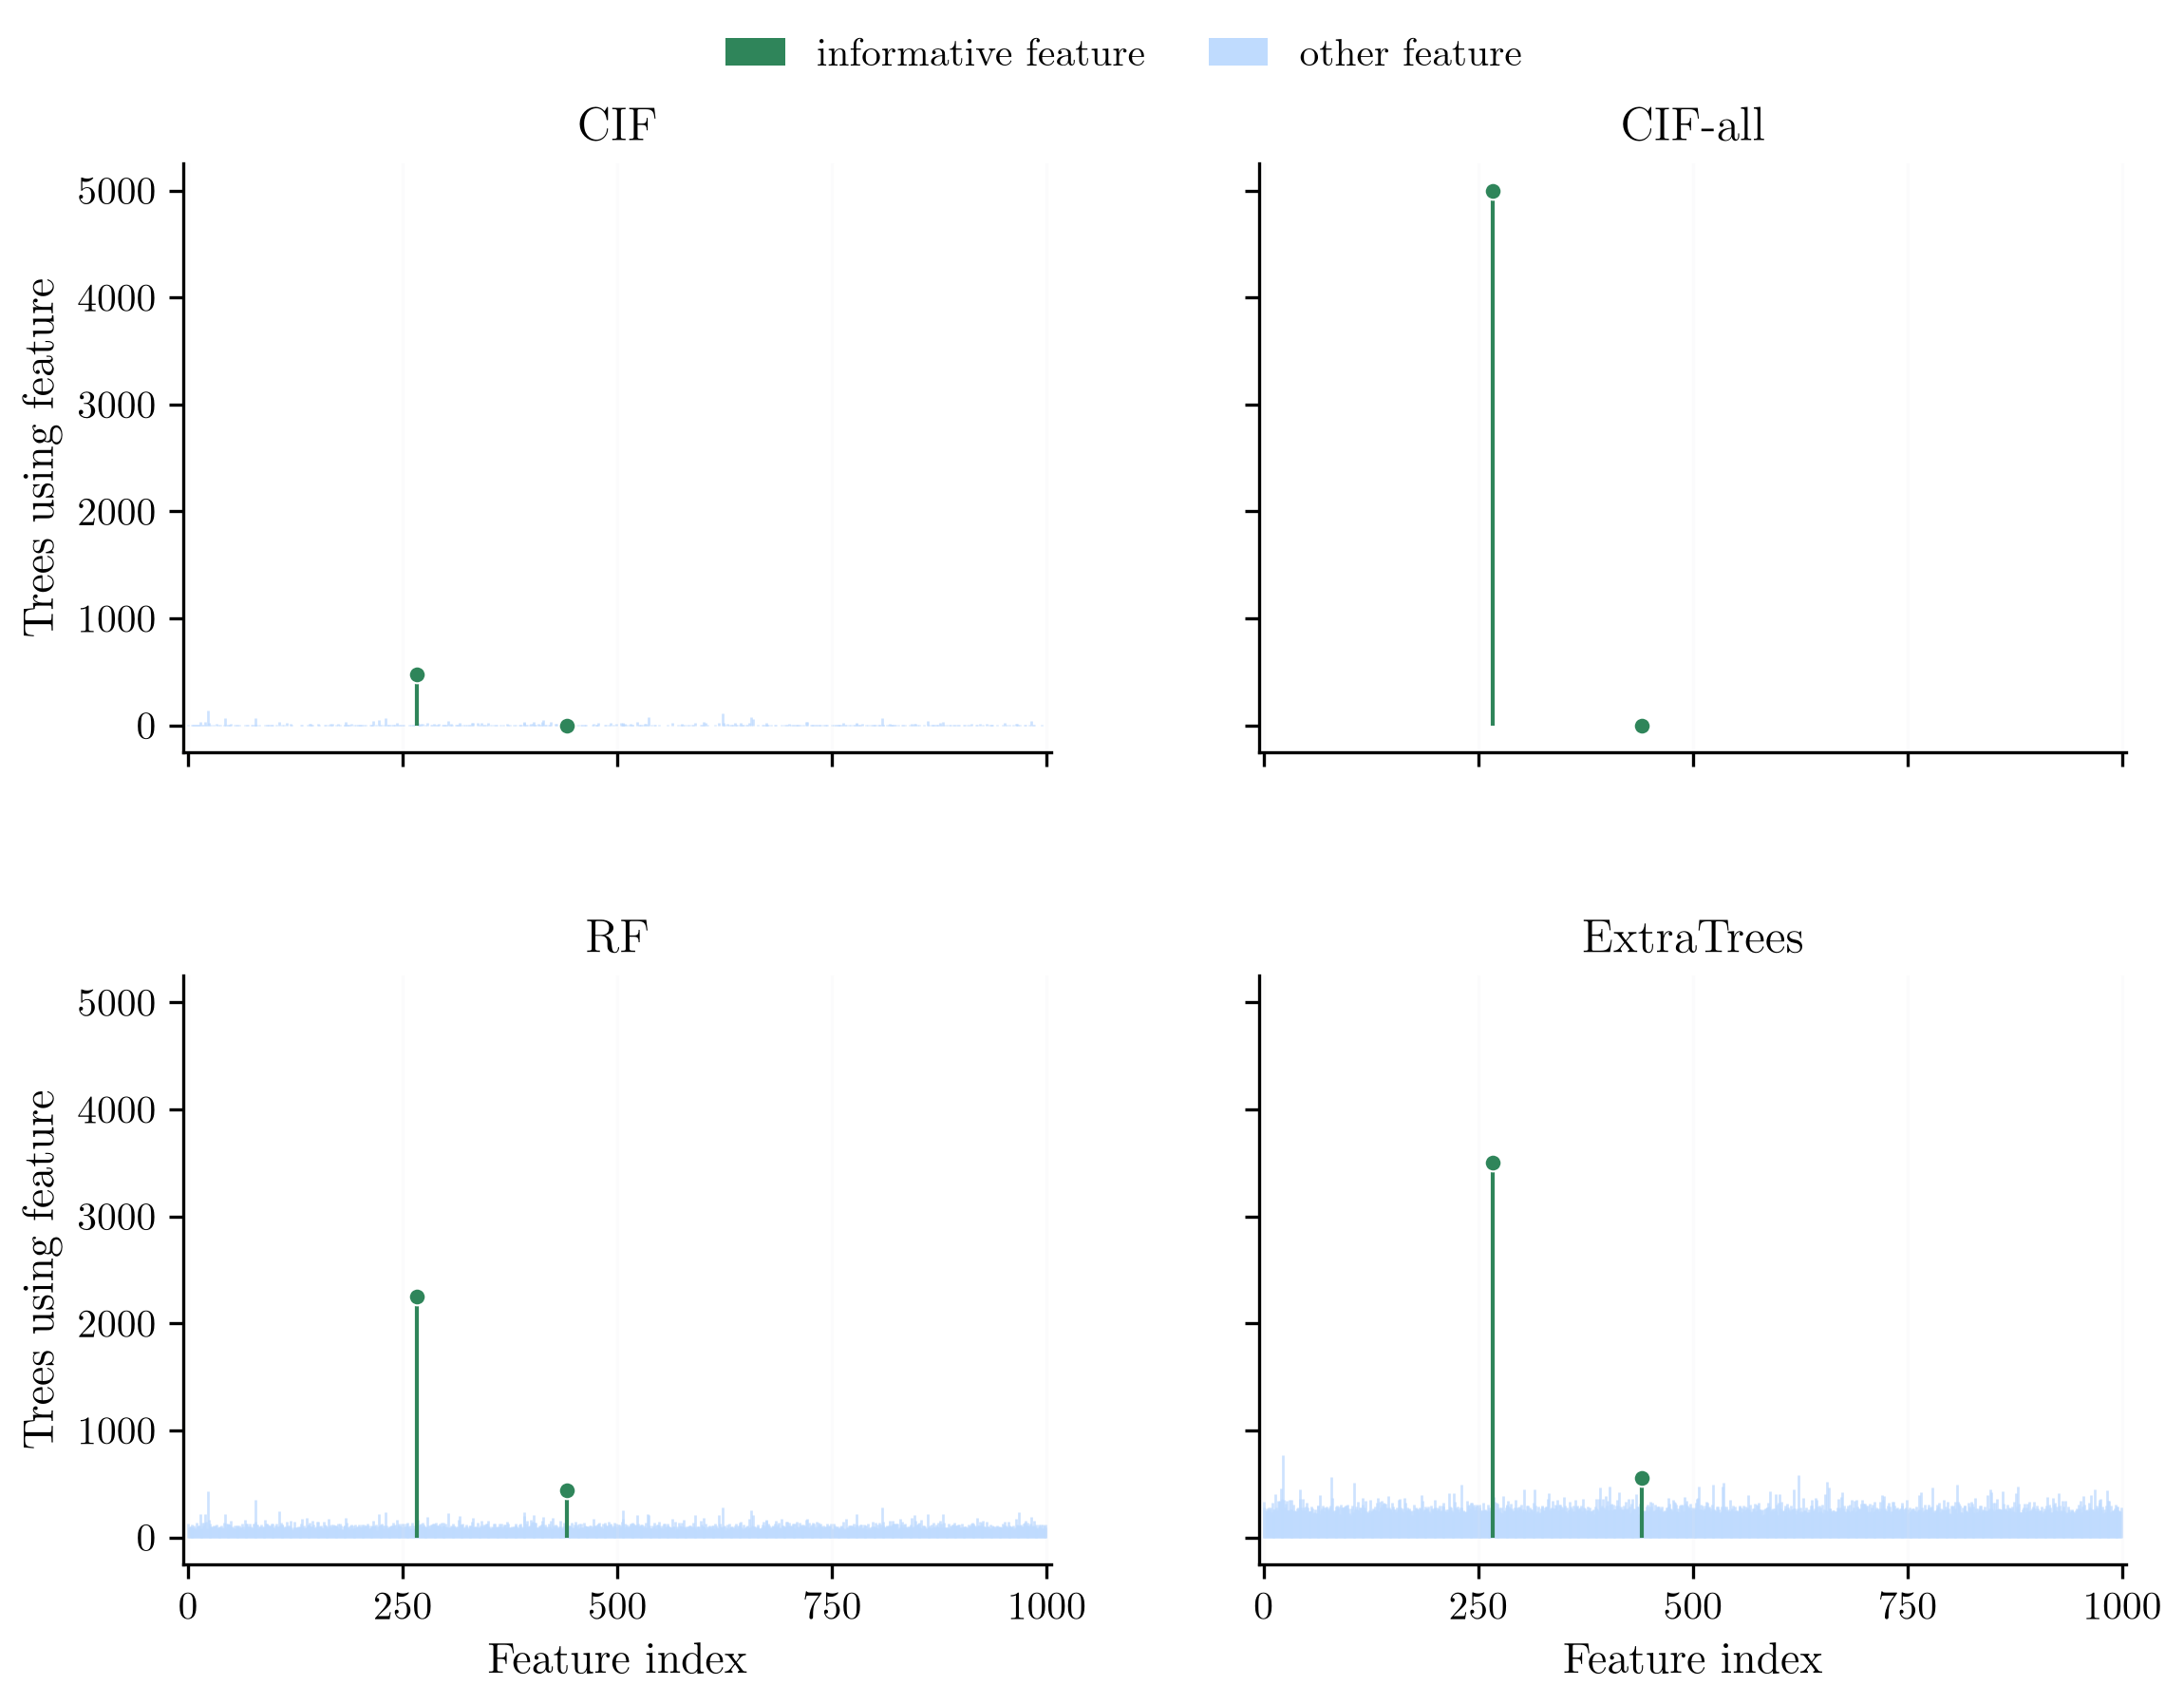
\includegraphics[width=0.84\linewidth]{figures/paper_mechanism_grid_forest_classification_feature_counts_p1000_i2_1000trees.png}
  \caption{Tree-level feature use in one sparse classification forest design
  ($n=250$, $p=1{,}000$, two informative features). Counts are the number of
  trees using each feature in at least one split, pooled over five fits of
  1,000 trees each, so the shared vertical axis runs to 5,000. CIF samples a
  subset of features at each node; CIF-all evaluates all nonconstant
  features.}
  \label{fig:candidate-forest-counts}
\end{figure}

\FloatBarrier
